\documentclass[tikz,border=2pt]{standalone}
\usepackage{tikz,amsmath}
\usetikzlibrary{arrows.meta, bending,calc,decorations.markings}
\newcommand{\bmR}{\boldsymbol{\mathcal{R}}}
\begin{document}
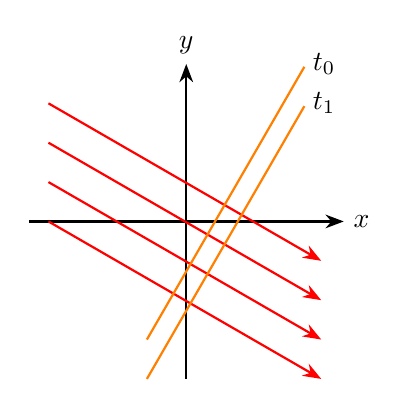
\begin{tikzpicture}[>=Stealth]

\draw [thick,->] (0,0) -- (4,0);
\node[right] at (4,0) {$x$};
\draw [thick,->](2,-2) -- (2,2);
\node[above] at (2,2) {$y$};

\foreach \y in {0, 0.5, 1.0, 1.5} {
        % Start at (0, \y), then move 4 units at a 30-degree angle
        \draw [thick, red,->] (0.25, \y) -- ++(-30:4);
    }

\foreach \y in {-2,-1.5} {
        % Start at (0, \y), then move 4 units at a 30-degree angle
        \draw [thick, orange] (1.5, \y) -- ++(60:4);
    }

\node at (3.75,2) {$t_0$};
\node at (3.75,1.5) {$t_1$};

%Angles



\end{tikzpicture}
\end{document}